\documentclass{standalone}

\usepackage{tikz}
\begin{document}

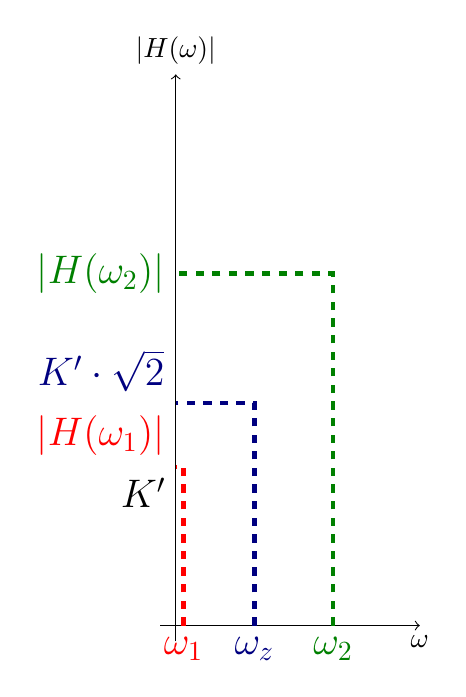
\begin{tikzpicture}[domain = 0:3, samples = 1000]
  \draw[->] (-0.2,0) -- (3.1,0) node[below] {$\omega$};
  \draw[->] (0,-0.2) -- (0,7) node[above] {$|H(\omega)|$};

  \draw[dashed,-,ultra thick,color=red] (0.1,0) node[font = \Large, below] {$\omega_1$} -- (0.1,2.009975) -- (0,2.009975) node[font = \Large, above left] {$|H(\omega_1)|$};
  \draw[dashed,-, ultra thick,color =blue!50!black] (1,0) node[font = \Large, below] {$\omega_z$} -- (1,2.828427) -- (0,2.828427) node[font = \Large, above left] {$K' \cdot \sqrt{2}$};
  \draw[dashed,-,ultra thick,color=green!50!black] (2,0) node[font = \Large, below] {$\omega_2$} -- (2,4.472136) -- (0,4.472136) node[font = \Large, left] {$|H(\omega_2)|$};
  \node[below left, font = \Large] at (0,2) {$K'$};
 \draw[ultra thick, color=black] plot[id=cero] function{2*sqrt(1+x**2)};

\end{tikzpicture}

\end{document}
